\documentclass[a4paper,11pt]{report}
\usepackage[T1]{fontenc}
\usepackage[utf8]{inputenc}
\usepackage{lmodern}
\usepackage{hyperref}
\usepackage{graphicx}
\usepackage{float}
\usepackage[english]{babel}

% title and subtitle
\title{\Huge \textbf{Unified Heteregeneous Networking Middleware Project Report}  \\ 
\huge \vspace{5mm} Fall 2015 }
% Author
\author{\textsc{Jincheng Li}}
\hypersetup{
  urlcolor=blue
}

\begin{document}

% \frontmatter
\maketitle

% Auto-generated table of contents, list of figures and list of tables %
\tableofcontents
% \mainmatter

\chapter{Introduction}
Devices with Internet access today are becoming increasingly mobile. The Heterogeneous Networking Middleware project provides a mechanism for devices to seamlessly handle network mobility, and make intelligent decisions about how and when to use different networks across multiple network interfaces. \\
The project started in 2012 in the IRT lab and went through significant development from 2012 to 2013. After a period of inactivity, it was restarted in Spring 2015 and continued until now (Fall 2015). \\
The prototype for this project started with a demo on Linux and focus is currently shifting to Android. In particular, this semester I focused on implementation of the demo in Android exclusively. Some work was done last semester to port the Linux implementation to Android, but there were issues with the provided C libraries on the Android platform. This semester we took a different approach and re-implemented some of the functionalities of the middleware within the Android Java Frameork. \\
In this report, I will cover existing work before I started contributing to the project, research done on Android framework's networking stack, and efforts toward implementing the middleware in Android. The text of this report and the code I wrote for this project are available at \url{https://github.com/jchli/hetnet-report}. See section 4.2.1 for details on how to obtain and work with the source code.

\chapter{Existing Work}
Prior to me being involved in the project, a lot of work has been done on the research on heterogeneous networks and Linux prototype implementation. Porting to Android started in Spring 2015. Here we briefly describe the various network protocols used in the project, and the Linux prototype implementation.

\section{Protocols}
There are three major protocols involved in the construction of the middleware: HIP, MIP, and MIH. HIP and MIP are two mobility protocols that achieve the same goal: ensuring continuous TCP connection in the presence of IP mobility. MIH is part of the IEEE 802.21 standard, providing an informational service that enables seamless handovers between heterogeneous layer-2 network technologies.

\subsection{IP Mobility}
We first introduce the idea of IP mobility. The internet was originally designed with the assumption that an IP address uniquely identifies a host. With multi-homing introduced and the proliferation of mobile internet devices which constantly move between different networks, this is no longer true. Currently, when an internet device switches between different network interfaces, consequently changing its IP address, the TCP (or any other transport protocol) connection in use will break because TCP identifies end-points with IP addresses. Given this, it is desirable to devise a mechanism that maintains the TCP connection when a device changes its IP address. \\
In both HIP and MIP, this is done through maintaining a unique identifier for a device even when the it changes its IP address. The details of how the identifier is defined and maintained varies for different protocols, but the idea stays the same.

\subsection{HIP}
\textbf{Description:} The Host Identity Protocol's approach to IP mobility introduces a Host Identity (HI) namespace based on a public key security infrastructure. Each host generates its own public key and uses the hash of that key as its identifier (or HIT - Host Identity Tag). This identifier encapsulates the host's varying IP address, and remains the same regardless of what new IP address the host obtains. Sockets are bound to HITs and therefore the connection does not break even if IP adderss changes. Using public keys has the added advantage of security - the host can conveniently prove its identity with a private-key signature. \\
HIP uses a 4-way handshake process to establish connection between two hosts. In its most general form, assuming both hosts are mobile (i.e. their IP addresses may change), a mobile host initiating the connection talks to the rendevzvous server (RVS) in order to reach the correspondent host. The RVS is responsible for keeping track of IP addresses and HITs of communicating hosts. Then the 4-way handshake process follows, which authenticates the two hosts, negotiates security parameters (through Diffie-Hellman exchange), and establishes ESP security associations (IPSec). The two hosts subsequently communicates through ESP payloads. When the IP address of a mobile host changes, HIP will initiate an update process to inform the other host (and RVS) of the change, so that the mapping from HITs to IP addresses can be updated and subsequent communcation sent to the new IP address. \\
\textbf{Implementation:} We are continuing to use the HIP for Linux implementation available at \url{http://infrahip.hiit.fi/}. It has experimental Android support and is being actively maintained.

\subsection{MIP}
\textbf{Description:} Mobile IP is another protocol for handling IP mobility. There are three main components in a MIP session: mobile node, home agent, and foreign agent. The mobile node is a device with internet connection that may roam between networks. The home agent is a router on the home network of the device, which serves as the anchor point for communication with the mobile node. The foreign agent is a router that may function as the point of attachment for the mobile node when it roams to a foreign network. \\
In MIP, the varying IP address of the mobile node is encapsulated in its home IP address, obtained from its home agent. Thus, to the outside world, the IP address of the mobile node will always be its home IP address. This is straightforward when the mobile node is on its home network - it simply assumes its home IP address. When the mobile node roams to a foreign network, it first obtains a new IP address called the care-of address. It then sends this information with a registration request to its home agent, which prompts the home agent to create a tunnel between itself and the foreign agent. Subsequently communication between the mobile node and its correspondent node will be tunneled between the home agent the foreign agent. Thus, the node will appear to have its home IP address, when in fact its IP address is the care-of address. \\
\textbf{Implementation:} We are not using MIP because after researching available implementations, we were not able to find any actively-maintained implementations of MIP available for Android.

\subsection{MIH}
\textbf{Description:} The IEEE 802.21 standard, also known as Media-Independent Handover Services, defines a set of services designed to allow for transparent service continuity during handovers between heterogeneous networks. It is an informational protocol in the sense that it only serves to provide information from various link types to a handover decision maker. It does not perform any network handovers or specify how handovers should be done. \\
MIH defines a logical entity called Media-Independent Handover Function (MIHF), which resides between the link layer and the network layer. MIHF provides services to entities at the network layer and above, called MIH Users (MIHUs), through Service Access Points (SAPs). These services include the following:
\begin{itemize}
\item Media-Independent Event Service \\
Reports events such as changes in link conditions.
\item Media-Independent Command Service \\
Enables MIHUs to issue commands to lower layers and manage the stream of events at lower layers. One example of an MIH command is \verb|MIH_Get_Link_Parameters|, which allows the MIHU to acquire the current paramter values of active links.
\item Media-Independent Information Service \\
Allows mobile nodes to obtain static information about available networks in its vicinity. This includes general information such as list of networks, their security and QoS support, and also PoA-specific information such as supported data rates, MAC layer types, etc.
\end{itemize}
MIHUs use information obtained from these services to make decisions about handover and link selection. In our case, the MIHU is the network manager within the middleware, which takes input from MIH, passes them on to the policy manager, which subsequently runs its algorithm to decide whether to make a network switch. \\
\textbf{Implementation:} Previously we used ODTONE / Open 802.21 as our implementation. This is perfectly fine for Linux. However, there is currently no support for Android. In addition, Android already provides some MIH-related functionalities within its Java framework. Thus instead of porting the ODTONE implementation to Android, our approach became investigating these functionalities in the Android framework, and then incorporating them into our prototype implementation.

\section{Linux Implementation}
We give a brief overview of the middleware's Linux implementation. This is mainly to provide an understanding of the existing implementation and serve as a reference for the implementation in Android.

\subsection{Architecture}
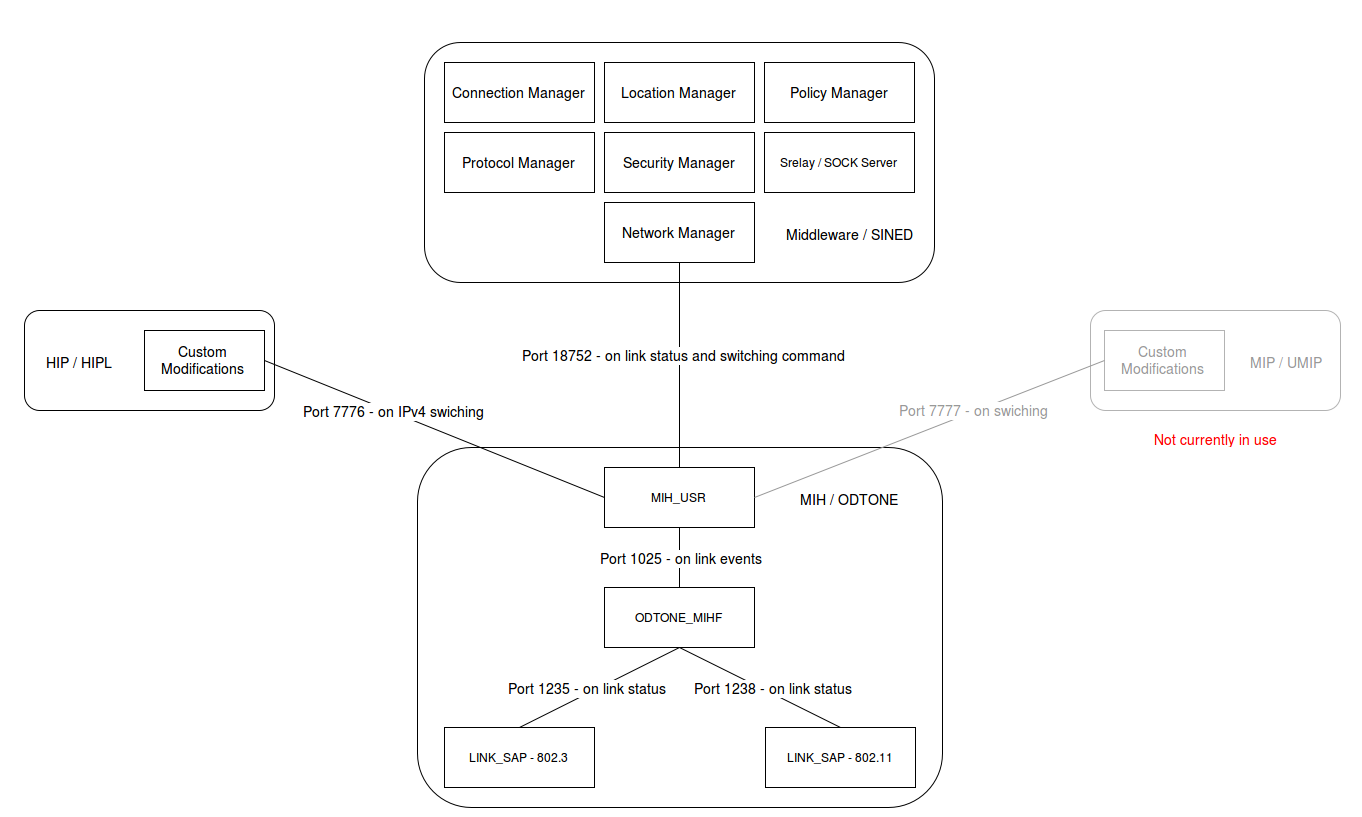
\includegraphics[width=\textwidth]{figures/linux_architecture.png} \\

The architecture of the Linux implementation has stayed the same as the previous semester. The middleware implements core functionalities including obtaining information from MIH, evaluating networks based on a policy model, making decisions to switch, and also security and authentication. MIH oversees the network interfaces, providing access to interface events and necessary information for the middleware to make a decision. It is also responsible for passing the command to switch interface, issued from the middleware, to HIP. HIP is ultimately responsible for making the network switch. This is done through custom modifications to HIP (done in the past), which forks a separate process from the main HIP process and handles the interface switch. 

\subsection{Comparison with Android}
The approach we took to an implementation in Android is largely concerned with the middleware component in this architecture, particularly the policy manager. We no longer need a lot of the machinery in this diagram because they are already provided by Android. For example, the network manager is responsible for communicating with MIH to obtain information about network interfaces. In the Android implementation, MIH information is already available in the framework, so it is no longer necessary to run a separate MIH process and obtain that information through sockets. Additionally, we no longer need to worry about how to make an interface switch, as it is also handled cleanly by Android. \\
However, we still need to port HIP to Android to allow for seamless handovers. As mentioned, HIP does not need to handle network switching anymore, so the custom modifications are no longer necessary. We can use HIPL's documentation on porting HIPL to Android and run the ported version for our system.

\chapter{Android Networking Stack}
In order to understand how Android performs intelligent network switching and the functionalities it provides similar to MIH, a fair amount of time was spent this semester researching the architecture of Android's networking stack. The idea is that once we understand the internal structure of Android's networking stack by looking at the source code, we can modify the source code to incorporate functionalities of our middleware into Android. We were able to map out the architecture of Android's network-related classes. Here we present the details of our findings. \\
Note that although there is some similar content in the Spring 2015 student report, the Android OS version studied there is 4.4 KitKat, whereas this document concerns 6.0 Marshmallow. Android introduced some intelligent network-switching functionality in between these two versions, and therefore there can be significant discrepancies between the network infrastructure of the two versions.

\section{Android OS Architecture}
We first introduce the architecture of the Android operating system. Broadly speaking, Android consists of five layers: Linux kernel, HAL, Android runtime + native libraries, Android Framework, and user applications. These five layers are laid out in the following diagram: % elaborate...

% android architecture diagram here
\begin{center}
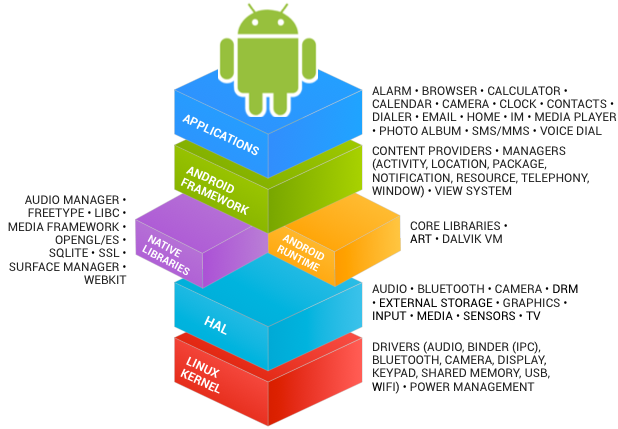
\includegraphics[scale=0.7]{figures/android_framework_details.png}
\end{center}

At the bottom of the Android software stack is the Linux kernel, which provides a level of abstraction between the device hardware and the upper layers of Android. The kernel provides typical low-level system services such as process, memory management, and also includes essential device drivers for hardware such as cellular and WiFi NICs. \\
The hardware abstraction layer (HAL) defines a standard interface for hardware vendors to implement and allows Android to be agnostic about lower-level driver implementations. We don't discuss HAL at any more length here as it is not vital for our purposes. \\
Next comes the Android runtime (i.e. Davlik VM) and native libraries, which are implemented in C/C++. The Dalvik VM is a virtual machine developed by Google to run Java applications on the Linux kernel. It is specifically designed for mobile devices and optimized for memory usage. The libraries at this layer include a subset of standard Java core libraries, and Android libraries including opengl, database (sqlite), webkit, etc. \\
Layered on top of the runtime and libraries is the Android Framework. This framework is implemented entirely in Java, and provides applications with an API that can be used to interact with system services, including UI, telephony, location, etc. This part of Android is what most of the research effort on Android this semester focused on. The Android demo also directly modifies Android Framework's source code to integrate our middleware functionalities into the system. \\
Finally on the top level are applications that interact directly with the user. These include native applications (web browser, settings, email) provided by Google and applications developed by third-party developers.

\section{Networking Stack}
Here we give an overview of Android's networking stack, including how Android structures its networking classes to manage the various aspects of networking, and how Android intelligently decides which networks to use. Later sections will go into details about the implementation of the networking stack. \\

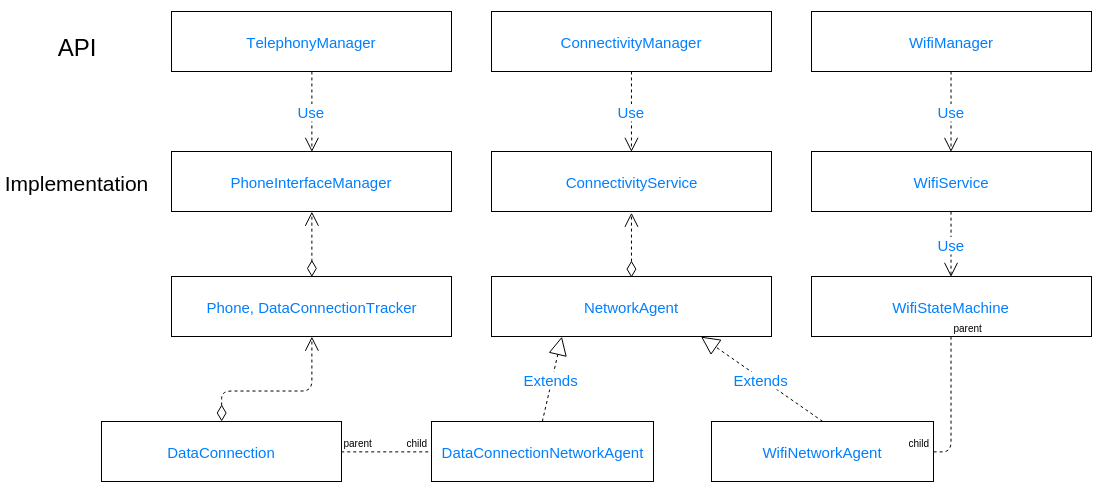
\includegraphics[scale=0.3]{figures/android_networking_stack.png}

There are roughly three layers in Android's networking stack (and incidentally, a lot of other components in the framework also adopt this architecture). The top layer has classes that export their methods as part of Android's API for application programmers. These classes typically have the `manager' suffix. The middle layer is Android's various services, which contains implementation logic for a lot of the methods that managers export. These services are long-running processes in the background that do not get interrupted by users switching between applications. Finally, the bottom layer, or any classes below the service layer, are specific implementations for different components of the Android framework. In the case of the networking stack, one very important class at this layer is \verb|NetworkAgent|. This class provides a common interface for different types of networks (e.g. WiFi, cellular), and enables \verb|ConnectivityService| to manage these networks uniformly. \\
The current version of Android allows applications to request networks with certain characteristics. These are true-false options that are detailed in the \verb|NetworkCapabilities| section below. When Android selects a network for an application, it first filters the list of available networks with the requested characteristics. If any characteristic does not match, the network is abandoned. Then, for all networks that pass the filter, it ranks these networks by their scores, and switches to the one with the highest score. Scoring for networks is managed differently for different types of networks. For WiFi networks, there is a scoring function within \verb|WifiStateMachine| that runs through several checks repeatedly, each time increasing/decreasing a network's score. For cellular networks, since there is usually only one such network, the scoring is very simple - it has either the maximum score or 0 depending on whether internet access has been verified.

\section{General Networking}
The following classes deal with network connectivity for all types of networks (cellular, WiFi, or ethernet). This is done through an abstraction called NetworkAgent that encapsulates different types of networks into a common interface, as is explained in more detail later in this section.

\subsection{ConnectivityManager}
Location: \verb|frameworks/base/core/java/android/net/|\\
As mentioned, classes with a ``Manager'' suffix are singleton classes exposed as part of the Android API for applications. Methods in these classes do not usually contain intricate program logic, but simply call some other system service class (e.g. methods in ConnectivityManager call corresponding methods in ConnectivtyService) which actually implements the required functionality. \\
\verb|ConnectivityManager| is reponsible for answering queries about the state of network connectivity, and for notifying applications about network connectivity changes. Additionally, it allows applications to request or select certain networks for their data traffic. This last feature is most relevant to our research, as it provides an entry point for applications to specify the characteristics of the network they prefer. The implementation of this feature is essentially a simplified version of the middleware's policy engine. An application can choose a policy for its network traffic, and Android will match the network that scores the highest according to that policy to this application. \\
The method invoked for applications to request certain networks is \verb|requestNetwork|, which takes as its input a \verb|NetworkRequest|, and a \verb|NetworkCallback|. As its name suggests, the \verb|NetworkCallback| is invoked once the network is switched to one that satisfies the request. The key component of a \verb|NetworkRequest| is a \verb|NetworkCapabilities| object, representing the capabilities of a network. This is elaborated more in the following subsection.

\subsection{NetworkCapabilities}
\verb|NetworkCapabilities| is the class currently used by Android to record information about a generic network. It contains a number of bit-mask fields indicating whether a network has a certain capability, and also a couple of numeric field such as bandwidth. Specifically, the class records the following capabilities about a network (categorization by myself):
\begin{enumerate}
\item services supported: \verb|MMS|, \verb|SUPL|, \verb|DUN|, \verb|FOTA|, \verb|IMS|, \verb|CBS|, \verb|WIFI_P2P|, \verb|IA|, \verb|RCS|, \verb|XCAP|, \verb|EIMS|
\item status: \verb|INTERNET|, \verb|NOT_RESTRICTED|, \verb|TRUSTED|, \verb|VALIDATED|
\item charateristics: \verb|NOT_METERED|, \verb|NOT_VPN|, \verb|CAPTIVE_PORTAL|
\item transport type: \verb|CELLULAR|, \verb|WIFI|, \verb|ETHERNET|, \verb|BLUETOOTH|, \verb|VPN|
\item bandwidth: \verb|LinkUpBandwidth|, \verb|LinkDownBandwidth|
\end{enumerate}
Note that for bandwidth, the numbers are currently an expected value instead of a measured statistic. \\
From the list above, we can see that for the most part the capabilities are binary. As such, the ``scoring'' function used by Android on \verb|NetworkCapabilities| is also straightforward: it simply filters out networks that do not satisfy certain capabilities (i.e. there is no score at this stage, it is only a binary filter). We will describe later how this works with another scoring mechanism that together decide which network is best suited to a \verb|NetworkRequest|.

\subsection{ConnectivityService}
Location: \verb|frameworks/base/services/core/java/com/android/server/| \\
\verb|ConnectivityService| provides implementations of many methods in \\ \verb|ConnectivityManager|. We discuss some of these methods relevant to our research below:
\begin{enumerate}
\item \verb|requestNetwork| \\
As mentioned, this is the method that applications invoke to request a network with the specified \verb|NetworkCapabilities|. The implementation of this method invokes the \verb|rematchNetworkAndRequests| method, which matches the best known network to the given request, and then after switching to that network, calls the given callback function.
\item \verb|rematchNetworkAndRequests| \\
This method is reponsible for matching the list of known networks to the list of network requests. Network requests include both default requests (e.g. cellular request, request for any network) and application-specific requests. The matching process is as follows: first, newtorks are filtered based on whether they have the specified capabilities, then, networks that pass through the filter are ranked by their scores, and if the one with the highest score is not the current network, a network switch to that network ensues. Also, if a network does not satisfy any requests, it is removed from the list of monitored networks. Network scores are computed in bearer-specific code (i.e. code managing a specific type of networks) and reported by \verb|NetworkAgent|. \verb|ConnectivityService| does not modify the scores of networks.
\item \verb|updateLinkProperties|, \verb|updateRoutes|, \verb|updateInterfaces| \\
These several update functions are the ``switching functions'' that we have been trying to locate. Internally they delegate the task of updating interfaces / routes to the network daemon, which passes commands down to the HAL layer, but in the Android framework, these are the functions that are responsible for switching between network interfaces. In fact, in our implementation of the demo, we don't ever call these functions directly. What we do instead is modify Android's scoring mechanism, and let Android handle the switching between networks.
\end{enumerate}

\subsection{NetworkAgent and NetworkAgentInfo}
Location: \verb|frameworks/base/core/java/android/com/server/connectivity/| \\
\verb|NetworkAgent| provides a common interface for different types of networks to report their status to \verb|ConnectivityService|. For example, it provides methods such as \verb|sendLinkProperties|, \verb|sendNetworkScore|, which gets called when there is a change in a network's properties or score. Subclasses optionally extend the methods of \verb|NetworkAgent| to deal with the specifics of a type of network. Updates by \verb|NetworkAgent| are done with a mesage-passing mechanism widely used in Android (dubbed the Looper framework, see \href{http://blog.coldflake.com/posts/Android-style-Message-Passing/}{this} relevant article). Thus \verb|ConnectivityService| does not directly interact with \verb|NetworkAgent|. Instead, \verb|NetworkAgentInfo| wraps around \verb|NetworkAgent|, storing the current status of a network (including its score), and enables \verb|ConnectivityService| to obtain information about all networks directly. One method of interest to us in \verb|NetworkAgentInfo.getCurrentScore|.

\section{WiFi Networks}
Android has a suite of classes built around managing WiFi networks. Compared to other types of networks, there are usually a long list of WiFi networks available, and the device needs to choose to connect to one of them (with the occasional help of users). Given this, Android implements algorithms to intelligently decide which WiFi network to use based network characteristics and past user preferences.

\subsection{WifiManager}
Location: \verb|frameworks/base/wifi/java/android/net/wifi/| \\
As with most manager classes, \verb|WifiManager| provides an API for Android applications, enabling them to manage all aspects of WiFi connectivity. Most of the relevant methods in \verb|WifiManager| have already been covered by the previous student report, so they are not repeated here. The following is an overview of the API that \verb|WifiManager| provides:
\begin{enumerate}
\item View and update the list of configured networks.
\item Connect or tear down a network. Query dynamic information about the currently active network.
\item Results of access point scans.
\item Defines Intent actions that are broadcast upon change in WiFi state (Intents are asynchronous messages that allow applications to request functionality from other Android components).
\end{enumerate}

\subsection{WifiStateMachine}
Location: \verb|frameworks/opt/net/wifi/service/java/com/android/server/wifi/| \\
\verb|WiFiStateMachine| implements the core logic of the WiFi subsystem. WiFi connectivity is managed as a state machine with around 24 states, examples of which are \verb|SupplicantStartingState|, \verb|ScanModeState|, \verb|ConnectModeState|, \verb|ObtainingIpState|, etc. Upon transitioning into a state, the state machine initiates some action (e.g. start scanning for networks, start dhcp). When the action completes, an event is typically triggered (e.g. scan result available, connected to network), and a message is sent back to the state machine, causing the state machine to transition into another state. \\
Notably, WiFi networks are scored by the \verb|calculateWifiScore| function in \verb|WifiStateMachine|. This function is routinely called to update the score of a network based on several statistics: the number of times the user turned off wifi to switch to LTE, the number of times the link is stuck (i.e. bad packet rate), the estimated link speed of the network, and the signal strength of the network.

\subsubsection{Scenario: Transitioning from LTE to WiFi}
Observing the sequence of events that happen when Android transitions from an LTE network to a WiFi network is very interesting and helped me understand a lot about how the WiFi subsystem works. We reproduce the sequence of events here for future reference. \\

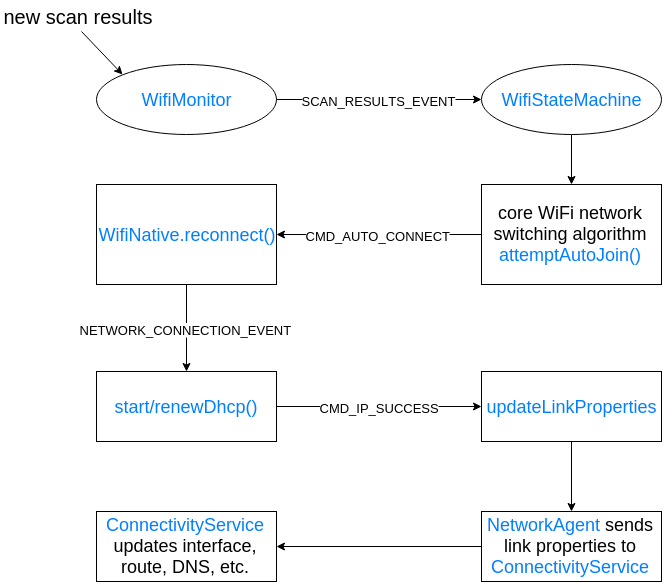
\includegraphics[scale=0.4]{figures/lte_to_wifi.png}

We assume here that the event that triggers the transition is the availability of new scan results, as opposed to, for instance, the user turning on the WiFi switch. When new scan results become available, the WiFi supplicant sends the event to \verb|WifiMonitor|, which then notifies \verb|WifiStateMachine| that new results are available. \verb|WifiStateMachine| receives this event in \verb|ConnectMode| (the mode it stays in when no WiFi networks are available to connect to), and subsequently attempts to connect to a network in the scan results. Here Android has to make a decision about which network to connect to. This is done with \verb|WifiAutoJoinController.attemptAutoJoin()|. We explain this in detail in the next subsection on the auto-join controller. Once \verb|attemptAutoJoin| decides which network to connect to, it sets that network as the default network, and delegates the task of actually connecting to it down to \verb|WifiNative|. Later, as the network is connected, a network connection event is triggered, sending \verb|WifiStateMachine| into \verb|ObtainingIpState|. Here the state machine starts the dhcp daemon, obtaining an IP address. Once done, it updates the corresponding link properties (properties recorded in the Android framework, not hardware properties). Finally, \verb|WifiNetworkAgent| sends the updated link properties to \verb|ConnectivityService|, which then calls its various update functions to update the interface, route, DNS, etc. This completes the switch to the new WiFi network.

\subsection{WifiAutoJoinController}
Location: \verb|frameworks/opt/net/wifi/service/java/com/android/server/wifi/| \\
The function \verb|attemptAutoJoin| in this class implements the core of a network switching algorithm. It runs through the list of networks, and for each network, considers several factors to decide whether it should be switched to. The factors include whether the user has selected this network before, the number of times we have attempted to join this network but failed, whether the network actually has internet access the last time we joined it, the signal strength of the network, the score of the network (as calculated by \verb|calculateWifiScore|), etc. It also considers special cases and handle with them accordingly. For example, when the user is using an application with streaming service (e.g. VoIP), it does not attempt to switch to a new network.

\section{Cellular Networks}

\subsection{TelephonyManager}
Location: \verb|frameworks/base/telephony/java/android/telephony/| \\
Unlike WiFi networks which are a stand-alone service, cellular networks are only a constituent of the telephony service. \verb|TelephonyManager| provides access to information about the various telephony services on the device. Applications can use the methods in this class to determine telephony services and states, as well as to access some types of subscriber information. Applications can also register a listener to receive notification of telephony state changes. The only methods relevant to our research in this class are \verb|setDataEnabled| and \verb|getDataEnabled|, which lets applications enable/disable cellular date, and obtain the state of the cellular connection.

\subsection{DataConnection}
Location: \verb|frameworks/base/telephony/src/java/com/android/internal|\\ \verb|/telephony/dataconnection/| \\
This class represents a single data connection via the cellular network. There may be multiple data connections and all of them are managed by the \verb|DcTracker|. \\
Similar to \verb|WifiStateMachine|, this class is also implemented as a state machine, attempting to establish connection to the cellular network. Most of the methods in this class deal with setting up the appropriate parameters for connecting to an access point, and recording the parameters internally (e.g. through \verb|updateLinkProperties|). These are already well documented in the previous student report. It is worth noting that there is not much scoring mechanism present. One internal class here is \verb|DcNetworkAgent|, which extends \verb|NetworkAgent|, and is responsible for sending characteristics about the cellular network to \verb|ConnectivityService|. However, \verb|sendNetworkScore| function of \verb|NetworkAgent| is never called here. Thus the score of a cellular network is simply its default score as implemented in \verb|NetworkAgentInfo.getCurrentScore|.

\chapter{Implementation in Android}

\section{Working with the Android Framework}
This section describes the necessary steps to set up and work with the Android framework. Most of this information can also be found on the Android Open-Source Project (AOSP: \url{https://source.android.com/source}) site. This guide documents the specific steps I went through, and any problems I encountered in the process.

\subsection{Environment Setup}

\subsubsection{Requirements}
Developing AOSP typically requires a 64-bit Linux or Mac OS system. I'm using 64-bit Linux Mint 17. As such, the following documentation applies to Linux only (note that Ubuntu should behave the same way as Linux Mint). For more reference on Mac OS, please refer to the AOSP site. Also note that 150 GB of free disk space is recommended for a single build.

\subsubsection{Establishing Build Environment}
Please see the page on AOSP (\url{https://source.android.com/source/initializing.html}) for reference on properly setting up dependencies for the build environment. These are simply some \verb|apt-get| commands and configurations. Note that at the end of the page there is a section called ``Optimizing a build environment'', which enables ccache to speed up recompilation. In my experience this was very helpful for saving compilation time. \\

\subsubsection{Downloading Android Source}
To download the Android source, you first need to have the \verb|repo| tool installed. This can be done with:
\begin{verbatim}
$ sudo curl https://storage.googleapis.com/git-repo-downloads/repo 
  > /usr/local/bin/repo
$ sudo chmod a+x /usr/local/bin/repo
\end{verbatim}
Next, create an empty directory to hold your working files:
\begin{verbatim}
$ mkdir ~/android
\end{verbatim}
Run \verb|repo init| to bring down the latest version of the \verb|repo| tool, and also supply it with a URL for the manifest, which specifies where the various repositories included in the Android source will be placed within your working directory.
\begin{verbatim}
$ repo init -u 
  https://android.googlesource.com/platform/manifest
\end{verbatim}
Note that this defaults to the \verb|master| branch, which is the one I developed on. At the time of writing, the Android version for the \verb|master| branch is 6.0 Marshmallow. It is also possible to download a different version of Android using a different manifest file. \\
Once the initialization is complete, run
\begin{verbatim}
$ repo sync
\end{verbatim}
to pull down the Android source tree. This should take anywhere between a couple hours to a day depending on your connection bandwidth. I believe it took approximately two hours with Columbia's public WiFi network. It is okay to interrupt the process. Running \verb|repo sync| again later will pick up from where the download was left off.

\subsection{Building and Running}
There are two ways to build/run the source code: with an emulator, or with a physical device. The emulator is a bit slow and lacks support for WiFi networks. It runs inside a QEMU hypervisor and has an emulated cellular connection. For physical devices, the only devices that AOSP currently supports are Nexus devices. Any other device requires a build configuration that's not directly available in the provided \verb|lunch| menu. You can find some useful information about non-Nexus device configurations on the CyanogenMod wiki (\url{https://wiki.cyanogenmod.org/w/Main_Page}).
\subsubsection{Building}
First, initialize the build environment by sourcing the \verb|envsetup.sh| script. Inside \verb|~/android| (where Android source is downloaded to), run
\begin{verbatim}
$ source build/envsetup.sh
\end{verbatim}
This includes several utility functions into the shell, which are necessary for building the source. Note that only \verb|bash| is compatible with these functions, so make sure you are not using another shell. \\
Next, choose a target to build with \verb|lunch|. You can see a list of possible targets by running \verb|lunch| without an argument, or you can choose a target directly with, for instance,
\begin{verbatim}
$ lunch aosp-arm_eng
\end{verbatim}
which builds the emulator with all debugging enabled. \\
Finally, build everything with \verb|make|. It is recommended to build using the \verb|-jN| argument, which parallelizes the build process. The fastest builds are ususally made with number of tasks N between 1 and 2 times the number of hardware threads on the computer. For example, for a computer with 8 cores, the fastest builds are between \verb|make -j8| and \verb|make -j16|.
\subsubsection{Running}
To run an emulator build, simply run \verb|emulator| in the terminal. To run a device-specific build, you can flash it onto the device with \verb|fastboot|. In order to flash a device, connect the device to your computer, and run
\begin{verbatim}
$ adb reboot bootloader
\end{verbatim}
which reboots the device into fastboot mode, and then run
\begin{verbatim}
$ fastboot flashall -w
\end{verbatim}
which flashes the system image onto the device.\\
For more information on running builds and choosing the appropriate build configuration for a device, see \url{https://source.android.com/source/running.html}.

\subsection{Developing}

\subsubsection{Repository Structure}
I found \href{http://stackoverflow.com/questions/9046572/how-to-understand-the-directory-structure-of-android-root-tree}{this} Stackoverflow post very useful in understanding what the purpose of the various directories in the Android repository. The following directories are most relevant to development:
\begin{itemize}
\item Build - files for the Android build system, including the \verb|envsetup.sh| script
\item Device - code for specific devices. This directory contains a lot of build configurations and scripts for different devices, including Nexus ones and emulators.
\item Frameworks - the bulk of the Android framework implemenation. This directory is composed of various stand-alone git repositories, which together are managed by \verb|repo|. Most of what we are working with can be found in the \verb|frameworks/base|, \verb|frameworks/opt/telephony|, \verb|frameworks/opt/net/wifi| projects.
\item Packages - contains source code for the default applications
\item Prebuilt - contains prebuilt binaries for convenience. These include cross-compilation toolchains, which can come in handy when porting HIP. Also included are device emulator binaries and Android Studio.
\item Out - build output directory.
\item (Kernel) - source for the Android kernel. Note that this is NOT part of the Android source download. In order to obtain the kernel, you have to download it separately. Also note that given the number of Android devices, the kernel source has a lot of versions, so be careful which version of the kernel you download.
\end{itemize}

\subsubsection{Repository Management}
As previously mentioned, \verb|repo| is used to manage development of the Android project. Development of a new topic branch typically starts with
\begin{verbatim}
$ repo start <BRANCH_NAME> [<PROJECT_LIST>]
\end{verbatim}
This will create a branch with the given name in each of the \verb|git| projects included in \verb|<PROJECT_LIST>|. Afterwards, simply proceed as usual to each of the projects, make some changes, and commit them separately with \verb|git|. You can use \verb|repo status [<PROJECT_LIST>]| to check the status of each of the projects. \\
Unfortunately there is no easy way to upload your changes to a remote repository. The \verb|repo| tool is designed to let you upload your changes to the Google source code server and submit them for review, eventually merging into the \verb|master| branch. However, since we are working on an experimental project with limited time, this is not a desired method. This is why I have saved my changes as \verb|patch| files for now. See section 4.2.1 below for more details.

\subsubsection{Testing}
Once changes are made, run the \verb|make -jN| command to build Android, and then either use the emulator or flash a physcial device to test the operating system. I have personally been testing the system on emulator only because there was no Nexus device with more than one type of network at my disposal. \\
There are two debugging tools that I found helpful with testing: \verb|adb logcat| and \verb|telnet|, which are detailed below.
\begin{enumerate}
\item When browsing Android code you will notice lots of logging lines. These system debug messages are stored in a buffer and can all be viewed and filtered with \verb|adb logcat|. The syntax for doing so is
\begin{verbatim}
$ adb logcat [filter-options]
\end{verbatim}
Every debug message has a tag and a priority. The tag is used to indicate which part of the system the message came from. This is frequently the name of the class where the message was collected from (e.g. ConnectivityService). There are a number of priorities for debugging messages: V (verbose), D (debug), I (info), W, (warning), E (error), F (fatal), S (silent). You can use a combination of tags and priorities to filter debug messages. For example, the following command
\begin{verbatim}
$ adb logcat ConnectivityService:* *:S
\end{verbatim}
prints all debug messages with the ConnectivityService tag, and silences all other messages.
\item The second useful debugging tool works with the emulator only. Each emulator instance provides a control console that you can connect to, to issue commands to that instance. If you are only running one emulator instance (as is usually the case), you can use \verb|telnet localhost 5554| to connect to the console. \\
The console provides several useful functionalities, among which is geo location provider emulation. Inside the console, you can issue commands such as \verb|geo fix <longitude> <latitude>| to send a fixed GPS location to the emulator. This can be particularly useful for our purposes since our policy vector consists of the location parameter.
\end{enumerate}

\newpage

\section{Android Demo Implementation}

\subsection{Source Code}
I have saved my changes to the Android source tree as \verb|patch| files and uploaded them to Github (\url{https://github.com/jchli/hetnet-report}). The rationale for doing this was explained in the ``Repository Management'' subsection above. After obtaining the source code of Android, you can apply the changes with the \verb|git am <patch file>| command within the appropriate directories in the Android framework. The two patch files are for the \verb|frameworks/base| project and the \verb|frameworks/opt/telephony| project, respectively. \\
For ease of finding the modifications, I have marked all the code I wrote with the \verb|// SINED| comment. I have also commented on any non-trivial code about its functionality. When navigating the code base it should be fairly easy to locate the changes I made, and to comprehend what the purpose of the code is. The following sections also give a detailed description of the changes. \\
List of classes I have modified:
\begin{itemize}
\item NetworkCapabilities (base)
\item NetworkRequest (base)
\item ConnectivityService (base)
\item NetworkAgentInfo (base)
\item DataConnection (opt/telephony)
\end{itemize}

\subsection{Design}
We first talk about the design of the demo implementation. Apart from the networking components that are already available in Android, there are three components of the middleware we need to be concerned with: the policy engine, HIP, and MIH. Our approach is to re-implement the policy engine in the Android framework, port the HIP implementation, and reuse the existing MIH functionality in Android. The first two choices are straightforward: since Android already provides a mechanism for applications to request networks with certain capabilities, it makes sense to extend on this to incorporate our policy engine; there are already successful efforts to port HIP for Linux to Android, so it also makes sense to use the ported version of HIPL for Android. For MIH, there is a choice between porting an MIH implementation and reusing what is available in Android. The caveat for using the MIH functionality available in Android is that Android does not have a unified MIH interface for all types of networks. Events from the WiFi subsystem is completely separate from events from the cellular network subsystem. This is usable, but complicates the implementation. Given that there is no successful port of MIH to Android yet, it seems desirable to reuse MIH components in Android. Note that the Multi-nets paper claim they have implemented a monitoring engine for Android (although their Android version is 4.3). This may be the MIH component we are looking for in Android. \\
We did not really end up incorporating the MIH functionality in Android. Instead we are using location as the only parameter of interest, and obtaining location information through a combination of \verb|LocationManager| and hard-coding (this information is what MIIS would provide). We give nearby networks a higher score, thus ranking them higher on the list of available networks. Android would then select the nearest network to connect to. 

\begin{center}
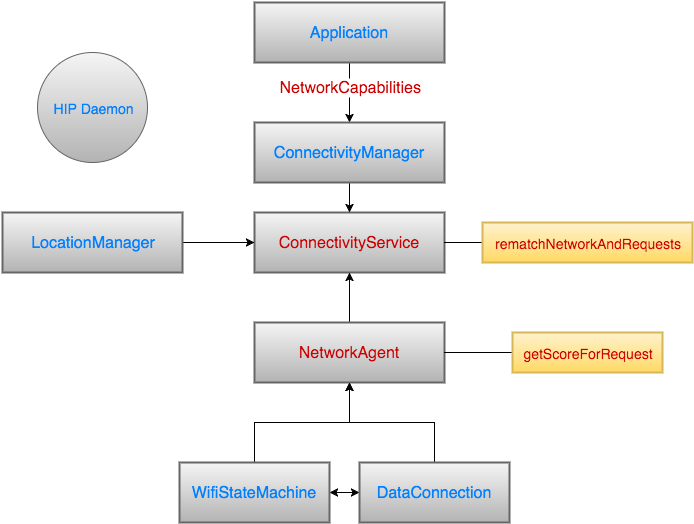
\includegraphics[scale=0.4]{figures/android_demo_design.png}
\end{center}

Above shows a diagram of our implementation design. Gray rectangles are classes, while yellow ones are methods. Entities marked red are ones being modified. We first enhance \verb|NetworkCapabilities| with the location parameter. Then, in \verb|NetworkAgent|, we implement an additional method called \verb|getScoreForRequest|, which matches network requests with the capabilities of the network, and calculates a score for the network based on its distance to the requested location. In \verb|ConnecitivtyService|, instead of scoring networks without reference to outstanding network requests, we use the new \verb|getScoreForRequest| function to score networks and rank them based on the extent to which they fulfill the current request. Thus the highest-ranked network will be the one nearest to the requested location, and Android will switch to that network. \\
Porting the HIP daemon is a separate task from implementation in the Android framework. I attempted to use a newer toolchain when cross-compiling the HIP code, with no success because of compilation errors. I then resorted to the porting script available from last semester's work, again to no avail. This time I was able to compile and load the binary onto Android, but Android keeps producing the following error:
\begin{verbatim}
error: only position independent executables (PIE) are supported.
\end{verbatim}
The cause of this appears to be a security feature in Android, which randomizes the address space of processes, making it difficult for attackers to exploit bugs in the program. I did not have enough time to investigate how to properly cross-compile HIP as a position-independent executable and load it onto Android.

\subsection{Implementation}
We show here some code snippets in my implementation. \\
\begin{figure}[H]
  \centering
  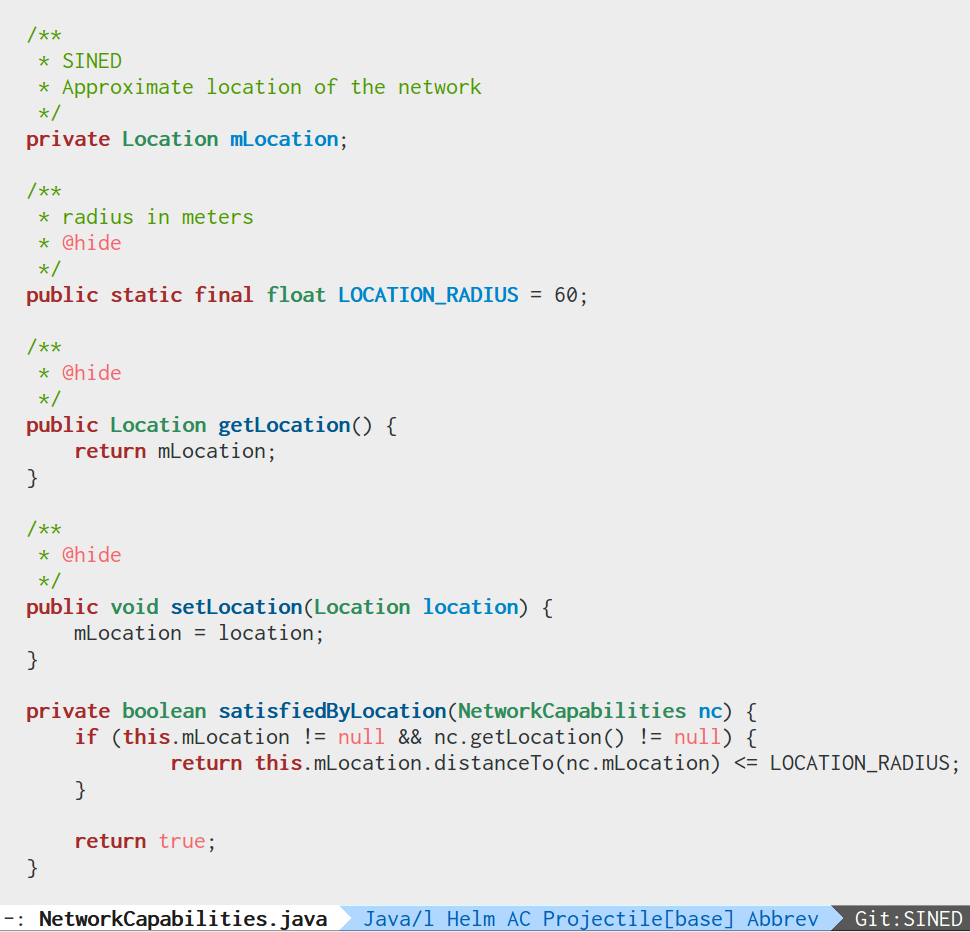
\includegraphics[scale=0.25]{figures/location.png}
  \caption{Enhancing NetworkCapabilities with Location}
\end{figure}
We add a location field to \verb|NetworkCapabilities|. The \verb|satisfiedByLocation| function checks if two networks are close to each other (i.e. within some constant radius). Since we have not tested the demo with a real device yet, the constant here has not been verified to work well. It may make sense to parameterize it on the signal strength of the network. \\
\begin{figure}[H]
  \centering
  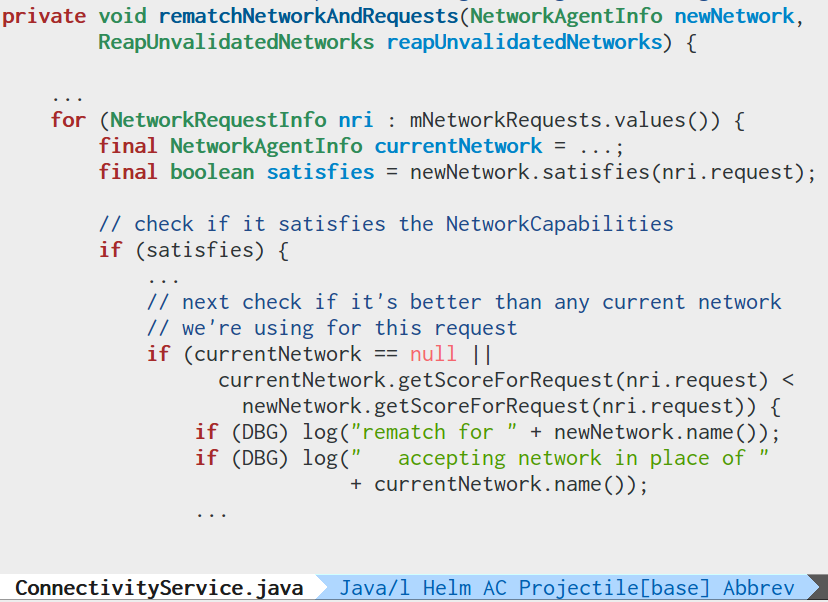
\includegraphics[scale=0.25]{figures/rematch.png}
  \caption{Ranking Networks by Request-based Scores}
\end{figure}
Figures 4.2 and 4.3 show the \verb|getScoreForRequest| function and its use in \verb|ConnectivityService|. We score networks on its distance to the requested location. If it is far away from the requested location, we apply a penalty to the network, otherwise we keep its score unchanged (existing scores are calculated by bearer-specific code).
\begin{figure}[H]
  \centering
  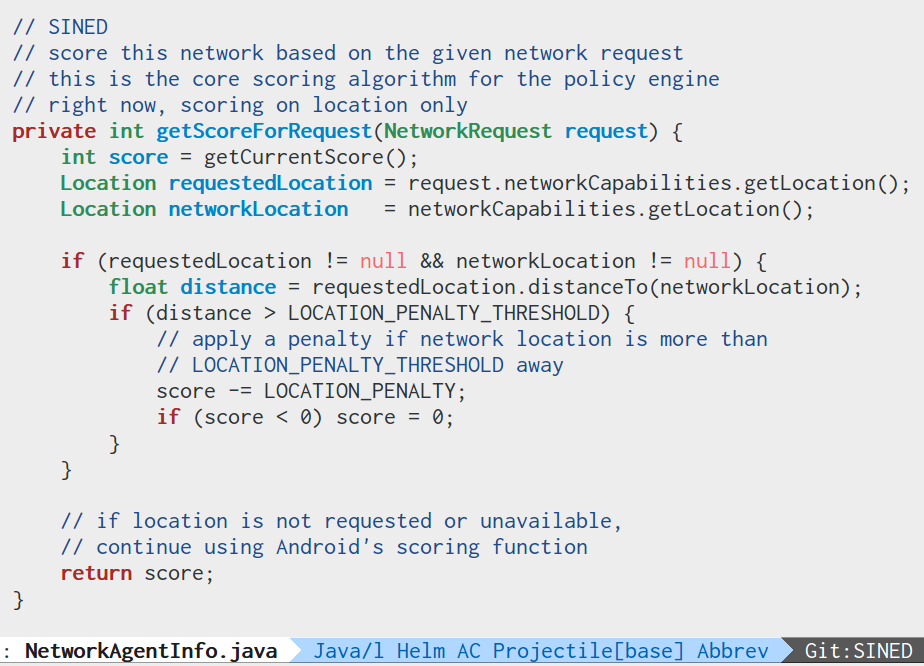
\includegraphics[scale=0.25]{figures/getScoreForRequest.png}
  \caption{getScoreForRequest}
\end{figure}
Finally, Figure 4.4 shows how we dynamically listen to location updates from \verb|LocationManager| and update the location of the default request. This ensures that we are always requesting for the network closest to the device.
\begin{figure}[H]
  \centering
  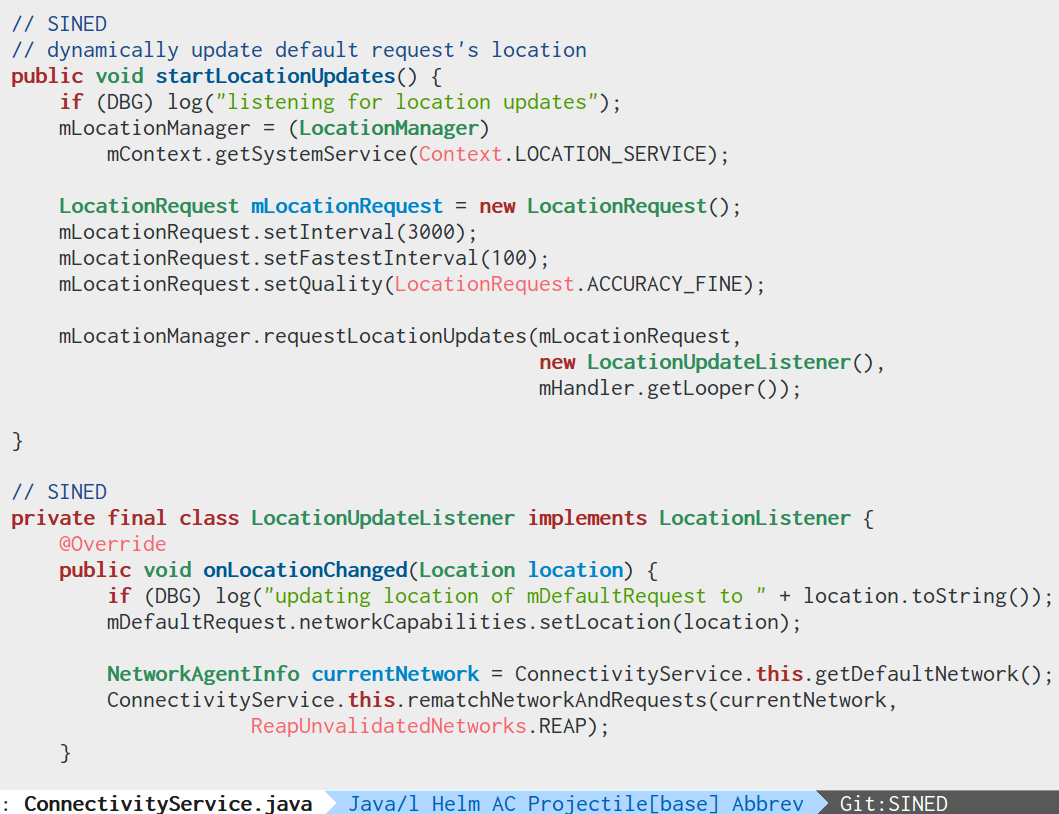
\includegraphics[scale=0.25]{figures/locationRequest.png}
  \caption{Updating Default Request to Current Location}
\end{figure}

\subsection{Future Work}
Continuing the implementation in Android, there are several tasks available:
\begin{itemize}
\item Make use of the MIH events in Android. Have middleware receive events about network availability / teardown, and act accordingly.
\item Enhance networks objects in Android with more statistics such as bandwidth, measured by testing download/upload link speed. Another possible approach is to develop a prototype for the MIIS database and query that database within Android.
\item Develop a full-fledged policy engine that considers several parameters and makes an intelligent decision about network choice.
\item Continue to work on cross-compiling HIPL to Android
\end{itemize}

\end{document}
